\documentclass[14pt]{extbook}
\usepackage{multicol, enumerate, enumitem, hyperref, color, soul, setspace, parskip, fancyhdr} %General Packages
\usepackage{amssymb, amsthm, amsmath, latexsym, units, mathtools} %Math Packages
\everymath{\displaystyle} %All math in Display Style
% Packages with additional options
\usepackage[headsep=0.5cm,headheight=12pt, left=1 in,right= 1 in,top= 1 in,bottom= 1 in]{geometry}
\usepackage[usenames,dvipsnames]{xcolor}
\usepackage{dashrule}  % Package to use the command below to create lines between items
\newcommand{\litem}[1]{\item#1\hspace*{-1cm}\rule{\textwidth}{0.4pt}}
\pagestyle{fancy}
\lhead{Progress Quiz 6}
\chead{}
\rhead{Version B}
\lfoot{9689-6866}
\cfoot{}
\rfoot{Spring 2021}
\begin{document}

\begin{enumerate}
\litem{
Determine the horizontal and/or oblique asymptotes in the rational function below.\[ f(x) = \frac{12x^{3} +41 x^{2} -40 x -48}{4x^{2} -13 x -12} \]\begin{enumerate}[label=\Alph*.]
\item \( \text{Oblique Asymptote of } y = 3x + 20. \)
\item \( \text{Horizontal Asymptote of } y = 4.0 \text{ and Oblique Asymptote of } y = 3x + 20 \)
\item \( \text{Horizontal Asymptote of } y = 3.0 \text{ and Oblique Asymptote of } y = 3x + 20 \)
\item \( \text{Horizontal Asymptote at } y = 4.0 \)
\item \( \text{Horizontal Asymptote of } y = 3.0  \)

\end{enumerate} }
\litem{
Which of the following functions \textit{could} be the graph below?
\begin{center}
    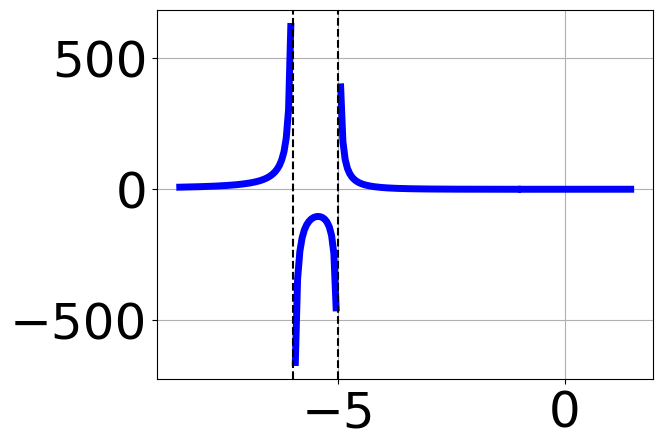
\includegraphics[width=0.5\textwidth]{../Figures/identifyGraphOfRationalFunctionB.png}
\end{center}
\begin{enumerate}[label=\Alph*.]
\item \( f(x)=\frac{x^{3} +4 x^{2} -4 x -16}{x^{3} +12 x^{2} +41 x + 30} \)
\item \( f(x)=\frac{x^{3} + x^{2} -4 x -4}{x^{3} +12 x^{2} +41 x + 30} \)
\item \( f(x)=\frac{x^{3} -1 x^{2} -4 x + 4}{x^{3} -12 x^{2} +41 x -30} \)
\item \( f(x)=\frac{x^{3} -1 x^{2} -4 x + 4}{x^{3} -12 x^{2} +41 x -30} \)
\item \( \text{None of the above are possible equations for the graph.} \)

\end{enumerate} }
\litem{
Determine the horizontal and/or oblique asymptotes in the rational function below.\[ f(x) = \frac{2x^{2} +x -6}{4x^{3} +4 x^{2} -9 x -9} \]\begin{enumerate}[label=\Alph*.]
\item \( \text{Oblique Asymptote of } y = 2x + 1. \)
\item \( \text{Horizontal Asymptote at } y = -2.000 \)
\item \( \text{Horizontal Asymptote of } y = 0.500  \)
\item \( \text{Horizontal Asymptote of } y = 0 \)
\item \( \text{Horizontal Asymptote of } y = 0.500 \text{ and Oblique Asymptote of } y = 2x + 1 \)

\end{enumerate} }
\litem{
Determine the vertical asymptotes and holes in the rational function below.\[ f(x) = \frac{12x^{3} +49 x^{2} -2 x -24}{12x^{2} +25 x + 12} \]\begin{enumerate}[label=\Alph*.]
\item \( \text{Holes at } x = -1.333 \text{ and } x = -0.75 \text{ with no vertical asymptotes.} \)
\item \( \text{Vertical Asymptotes of } x = -1.333 \text{ and } x = -0.75 \text{ with no holes.} \)
\item \( \text{Vertical Asymptote of } x = -1.333 \text{ and hole at } x = -0.75 \)
\item \( \text{Vertical Asymptote of } x = 1.0 \text{ and hole at } x = -0.75 \)
\item \( \text{Vertical Asymptotes of } x = -1.333 \text{ and } x = 0.667 \text{ with a hole at } x = -0.75 \)

\end{enumerate} }
\litem{
Which of the following functions \textit{could} be the graph below?
\begin{center}
    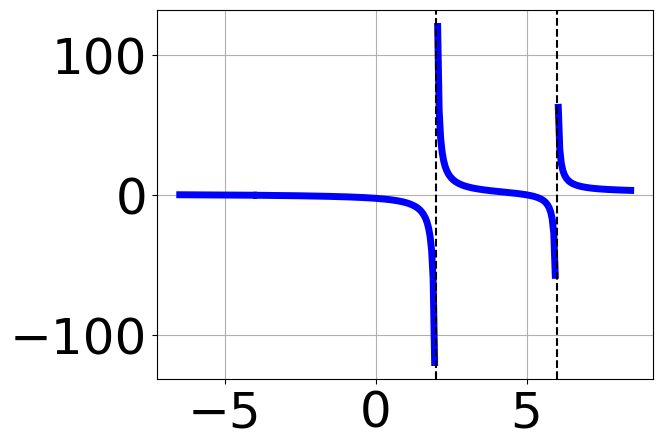
\includegraphics[width=0.5\textwidth]{../Figures/identifyGraphOfRationalFunctionCopyB.png}
\end{center}
\begin{enumerate}[label=\Alph*.]
\item \( f(x)=\frac{x^{3} -7 x^{2} -16 x + 112}{x^{3} -4 x^{2} -17 x + 60} \)
\item \( f(x)=\frac{x^{3} -7 x^{2} -16 x + 112}{x^{3} -4 x^{2} -17 x + 60} \)
\item \( f(x)=\frac{x^{3} +12 x^{2} +39 x + 28}{x^{3} +4 x^{2} -17 x -60} \)
\item \( f(x)=\frac{x^{3} +7 x^{2} -16 x -112}{x^{3} +4 x^{2} -17 x -60} \)
\item \( \text{None of the above are possible equations for the graph.} \)

\end{enumerate} }
\litem{
Determine the vertical asymptotes and holes in the rational function below.\[ f(x) = \frac{16x^{3} -16 x^{2} -81 x -45}{12x^{2} -11 x -15} \]\begin{enumerate}[label=\Alph*.]
\item \( \text{Vertical Asymptotes of } x = 1.667 \text{ and } x = -0.75 \text{ with no holes.} \)
\item \( \text{Vertical Asymptote of } x = 1.333 \text{ and hole at } x = -0.75 \)
\item \( \text{Holes at } x = 1.667 \text{ and } x = -0.75 \text{ with no vertical asymptotes.} \)
\item \( \text{Vertical Asymptote of } x = 1.667 \text{ and hole at } x = -0.75 \)
\item \( \text{Vertical Asymptotes of } x = 1.667 \text{ and } x = -1.25 \text{ with a hole at } x = -0.75 \)

\end{enumerate} }
\litem{
Determine the horizontal and/or oblique asymptotes in the rational function below.\[ f(x) = \frac{6x^{3} +47 x^{2} +112 x + 80}{2x^{2} -x -15} \]\begin{enumerate}[label=\Alph*.]
\item \( \text{Horizontal Asymptote of } y = 3.0  \)
\item \( \text{Horizontal Asymptote of } y = 3.0 \text{ and Oblique Asymptote of } y = 3x + 25 \)
\item \( \text{Horizontal Asymptote of } y = 3.0 \text{ and Oblique Asymptote of } y = 3x + 25 \)
\item \( \text{Oblique Asymptote of } y = 3x + 25. \)
\item \( \text{Horizontal Asymptote at } y = 3.0 \)

\end{enumerate} }
\litem{
Determine the vertical asymptotes and holes in the rational function below.\[ f(x) = \frac{9x^{3} +9 x^{2} -10 x -8}{9x^{2} -3 x -20} \]\begin{enumerate}[label=\Alph*.]
\item \( \text{Vertical Asymptote of } x = 1.667 \text{ and hole at } x = -1.333 \)
\item \( \text{Vertical Asymptotes of } x = 1.667 \text{ and } x = -0.667 \text{ with a hole at } x = -1.333 \)
\item \( \text{Holes at } x = 1.667 \text{ and } x = -1.333 \text{ with no vertical asymptotes.} \)
\item \( \text{Vertical Asymptotes of } x = 1.667 \text{ and } x = -1.333 \text{ with no holes.} \)
\item \( \text{Vertical Asymptote of } x = 1.0 \text{ and hole at } x = -1.333 \)

\end{enumerate} }
\litem{
Determine the vertical asymptotes and holes in the rational function below.\[ f(x) = \frac{6x^{3} -1 x^{2} -11 x + 6}{4x^{2} +16 x + 15} \]\begin{enumerate}[label=\Alph*.]
\item \( \text{Vertical Asymptotes of } x = -2.5 \text{ and } x = 0.667 \text{ with a hole at } x = -1.5 \)
\item \( \text{Vertical Asymptotes of } x = -2.5 \text{ and } x = -1.5 \text{ with no holes.} \)
\item \( \text{Holes at } x = -2.5 \text{ and } x = -1.5 \text{ with no vertical asymptotes.} \)
\item \( \text{Vertical Asymptote of } x = -2.5 \text{ and hole at } x = -1.5 \)
\item \( \text{Vertical Asymptote of } x = 1.5 \text{ and hole at } x = -1.5 \)

\end{enumerate} }
\litem{
Determine the horizontal and/or oblique asymptotes in the rational function below.\[ f(x) = \frac{4x^{2} -3 x -10}{24x^{3} -14 x^{2} -35 x + 25} \]\begin{enumerate}[label=\Alph*.]
\item \( \text{Horizontal Asymptote of } y = 0 \)
\item \( \text{Horizontal Asymptote of } y = 0.167  \)
\item \( \text{Horizontal Asymptote at } y = 2.000 \)
\item \( \text{Horizontal Asymptote of } y = 0.167 \text{ and Oblique Asymptote of } y = 6x + 1 \)
\item \( \text{Oblique Asymptote of } y = 6x + 1. \)

\end{enumerate} }
\end{enumerate}

\end{document}